\documentclass{standalone}

\usepackage{tkz-euclide}

\begin{document}
	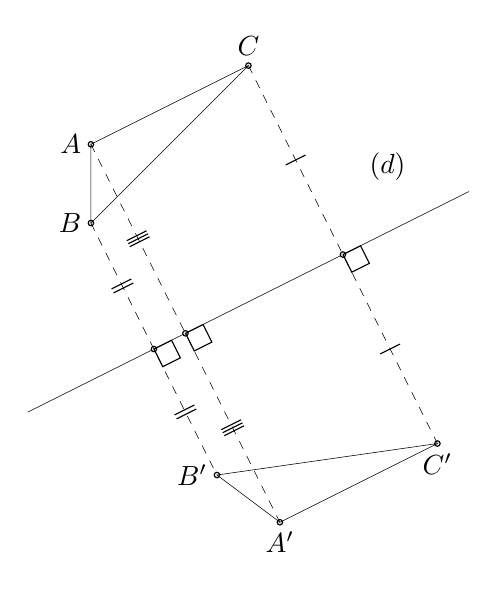
\begin{tikzpicture}
		\tkzInit[xmin=-2,xmax=6,ymin=-4,ymax=4]
		%\tkzDrawX
		%\tkzDrawY
		\tkzDefPoint(0,0){O}
		\tkzDefPoint(4,2){P}
		
		\tkzDefPoints{0/3/A, 0/2/B, 2/4/C}
		\tkzDefPointBy[reflection=over O--P](A)\tkzGetPoint{A'}
		\tkzDefPointBy[reflection=over O--P](B)\tkzGetPoint{B'}
		\tkzDefPointBy[reflection=over O--P](C)\tkzGetPoint{C'}
		\tkzInterLL(O,P)(A,A')\tkzGetPoint{I}
		\tkzInterLL(O,P)(B,B')\tkzGetPoint{J}
		\tkzInterLL(O,P)(C,C')\tkzGetPoint{K}
		
		\tkzDrawLine(O,P)
		\tkzLabelLine[above right=2](O,P){$(d)$}
		
		\tkzDrawPoints(A,I,A')
		\tkzDrawSegment[dashed](A,A')
		\tkzMarkRightAngle(A',I,P)
		
		\tkzLabelPoints[left](A)
		\tkzLabelPoints(A')
		\tkzMarkSegments[mark=|||](A,I I,A')

		\tkzDrawPoints(B,J,B')
		\tkzDrawSegments[dashed](B,B')
		\tkzMarkRightAngle(B',J,P)
		
		\tkzLabelPoints[left](B)
		\tkzLabelPoints[left](B')
		\tkzMarkSegments[mark=||](B,J J,B')
		
		\tkzDrawPoints(C,K,C')
		\tkzDrawSegments[dashed](C,C')
		\tkzMarkRightAngle(C',K,P)
		
		\tkzLabelPoints[above](C)
		\tkzLabelPoints(C')
		\tkzMarkSegments[mark=|](C,K K,C')
		
		\tkzDrawPolygons(A,B,C A',B',C')
	\end{tikzpicture}
\end{document}